\documentclass[letterpaper, oneside, 11pt]{book}
\usepackage[left=1in, right=1in, top=0.75in]{geometry}
\usepackage[svgnames]{xcolor}
\usepackage{float}
\usepackage{graphicx}
\usepackage{setspace}
\usepackage{acronym}
\usepackage[sfdefault]{roboto}
\usepackage{xcolor}
\usepackage{sectsty}
\usepackage[colorlinks=true, linkcolor=gray]{hyperref}
\usepackage[utf8]{inputenc}
\usepackage{hyperref}
\definecolor{MyBlue}{rgb}{0.03, 0.27, 0.49}
\chapterfont{\color{MyBlue}}
\sectionfont{\color{MyBlue}}
\subsectionfont{\color{MyBlue}}

\begin{document}
%%========================================================================
\begin{titlepage}
	\raggedleft
	\begin{figure}[H]
	\centering
		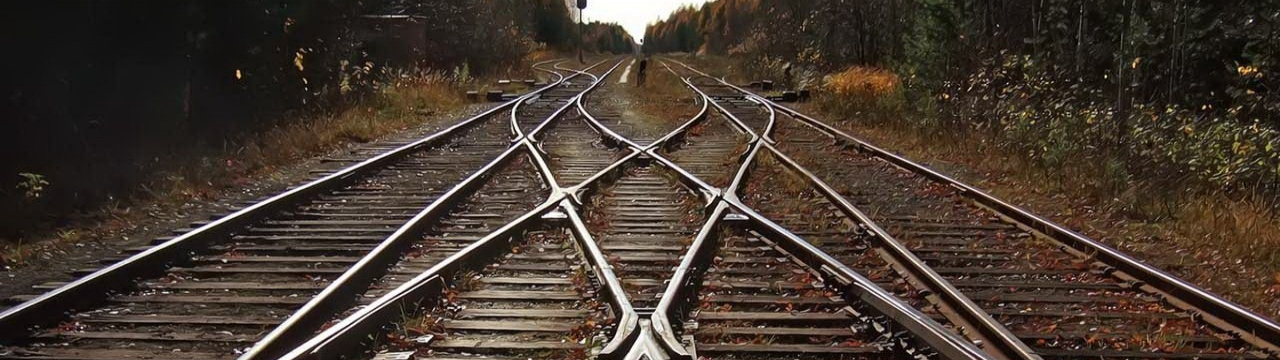
\includegraphics[scale=1.53]{railway_track.jpg}
	\label{fig:track}
\end{figure}
	\vspace*{0.167\textheight}
	\textbf{\LARGE System Design and Implementation}\\[\baselineskip]
    \textbf{\textcolor{MyBlue}{\Huge R\Large ailway \Huge A\Large dministration and \Huge I\Large nformation \Huge L\Large ogical \Huge S\Large ystem}}\\[\baselineskip]
	{\Large \textit{RAILS for Model Railroads}}
	\vfill
    \vspace*{\baselineskip}
	{\small David Bristow}

	{\small Version 1.0.1}
	
	{\small Jun 8, 2023}
	\vspace*{3\baselineskip}
\end{titlepage}
%%========================================================================
\tableofcontents
%% copyright notice
%%========================================================================
\chapter{Microcontrollers for RAILS}
\section{Introduction}
\gls{rails} is a software model and implementation of an automated system to assist the model railroader achieve realism in the operation of a model railroad.
There are four user interface \gls{spa} that provide different aspects of rails they are:
\begin{itemize}
  \item \gls{rsrm} allows the user to match a rfid tag to a rollingstock's road name and number;
  \item \gls{mrim} allows the user to create, update and delete model railroad assets, such as rolling stock;
  \item \gls{mppm} allows the user to enter information about their projects and purchases; and
  \item \gls{mrlm} allows the user to enter information about their layout and control elements of it.
\end{itemize}
\section{RSRM Components}
The implementation of \gls{rsrm} consists of the following micro-services components:
\begin{itemize}
\item \gls{rfid} Controller is a micro-controller that processes \gls{rfid} tags obtained from a \gls{rfid} reader and then publishes \gls{iot} messages to the \gls{mqtt} Broker;
\item \gls{mqtt} Broker is responsible for receiving \gls{rfid} and micro info messages, filtering them, posting to designated topics and sending messages to clients subscribing to topics. The subscribers and publishers bridge the \gls{mqtt} elements with the GUI applications. The broker handles \gls{iot} messages;
\item \gls{isrs} subscribes to \gls{rfid} messages and pushes them via a web-socket to the rsm component;
\item \gls{isms} that subscribes to micro controller startup and heartbeat messages, updating the micros collection via \gls{rlds};
\item \gls{rlds} provides \gls{rest} access to model railroad layout collections including micros;
\item \gls{rids} provides \gls{rest} access to railroad inventory collections including rollingstock;
\item MongoDB a NoSQL database program that stores data records as documents which are gathered in collections. A database stores one or more collections of documents;
\item \gls{mr} Data is the document repository, used by MongoDB, to store complete collections of items such as rollingstock, industries (producers and consumers), track elements, turnouts, projects, purchases, etc. in support of \gls{rails}; and
\item \gls{rsrm} is the \gls{spa} that allows a user to match a \gls{rfid} tag to a rollingstock's road name and number.
\end{itemize}
Figure \ref{fig:rsms-ms-components} depicts the micro-services used to create the rolling stock \gls{rfid} management subsystem.

\begin{figure}[H]
	\centering
		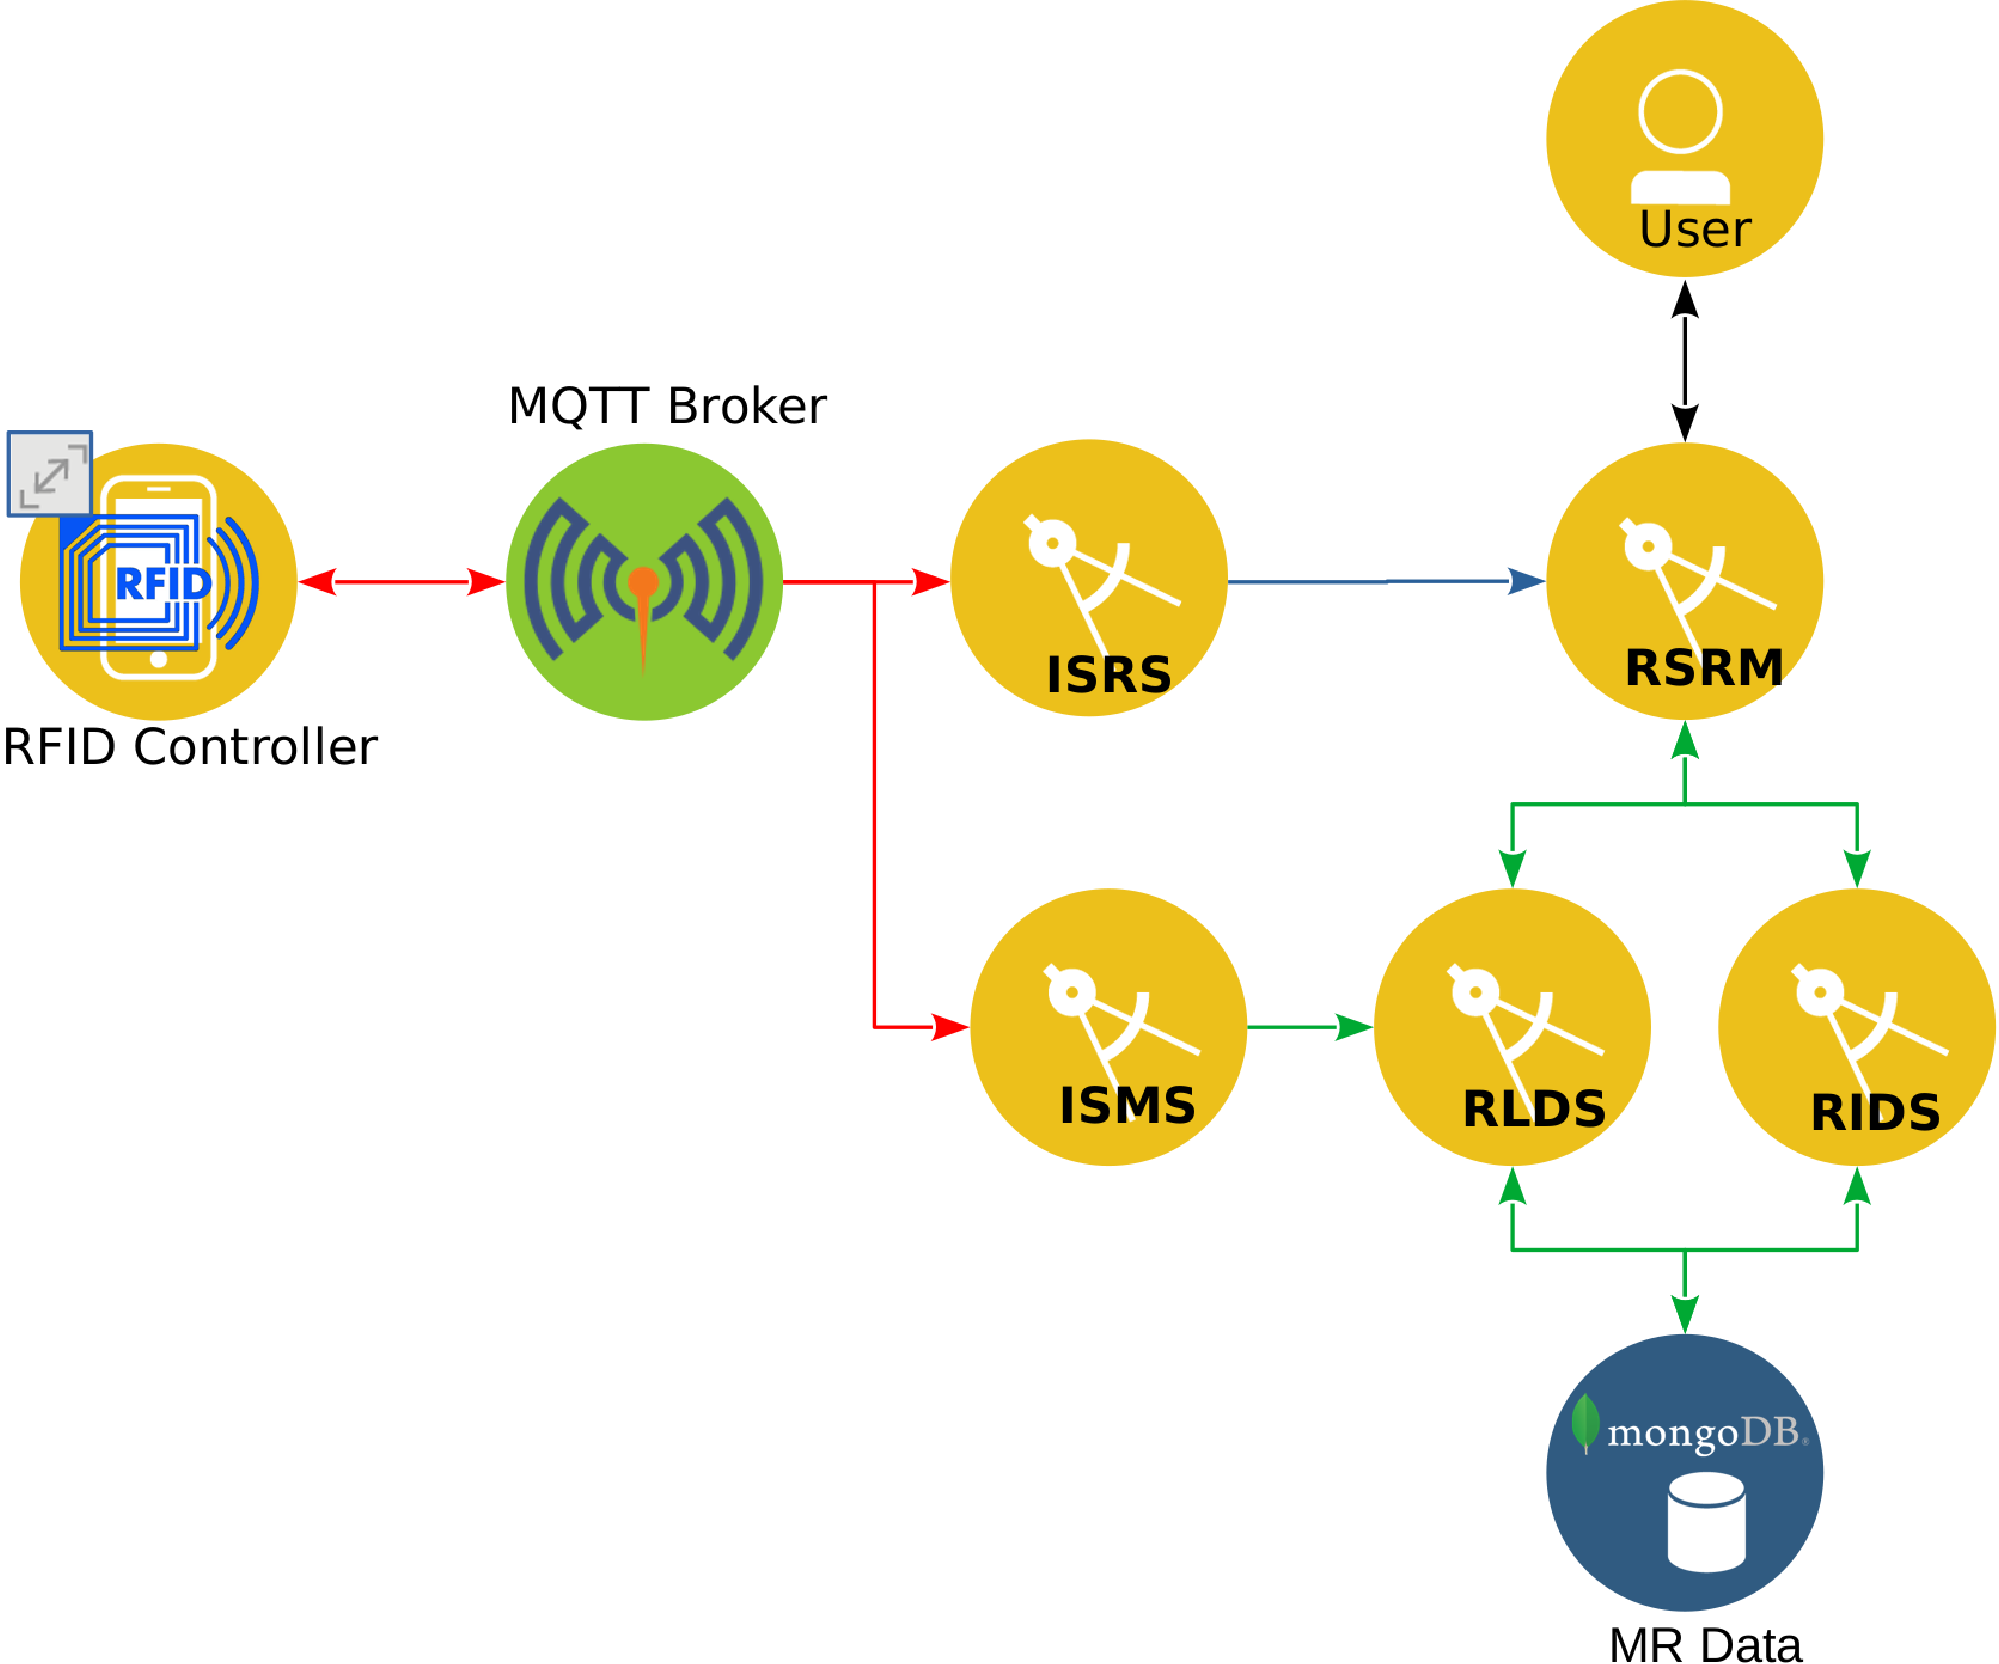
\includegraphics[scale=0.15]{../Images/rsms_microservices.png}
	\caption{Microservices Components}
	\label{fig:rsms-ms-components}
\end{figure}

Three system components that make up this subsystem:
\begin{itemize}
\item \gls{rfid} Controller is a micro-controller that processes \gls{rfid} tags obtained from a \gls{rfid} reader and then publishes \gls{iot} messages to the \gls{mqtt} Broker;
\item Network is a \gls{tcpip} communication medium that connects the \gls{rfid} Controller, \gls{mqtt} Broker and \gls{rsrm} components; and
\item Host is a computer that runs the \gls{mqtt} Broker and other \gls{rsrm} micro-services components.
\end{itemize}
Figure \ref{fig:rsms-system} depicts the systems components used to create the rolling stock \gls{rfid} management subsystem.

\begin{figure}[H]
	\centering
		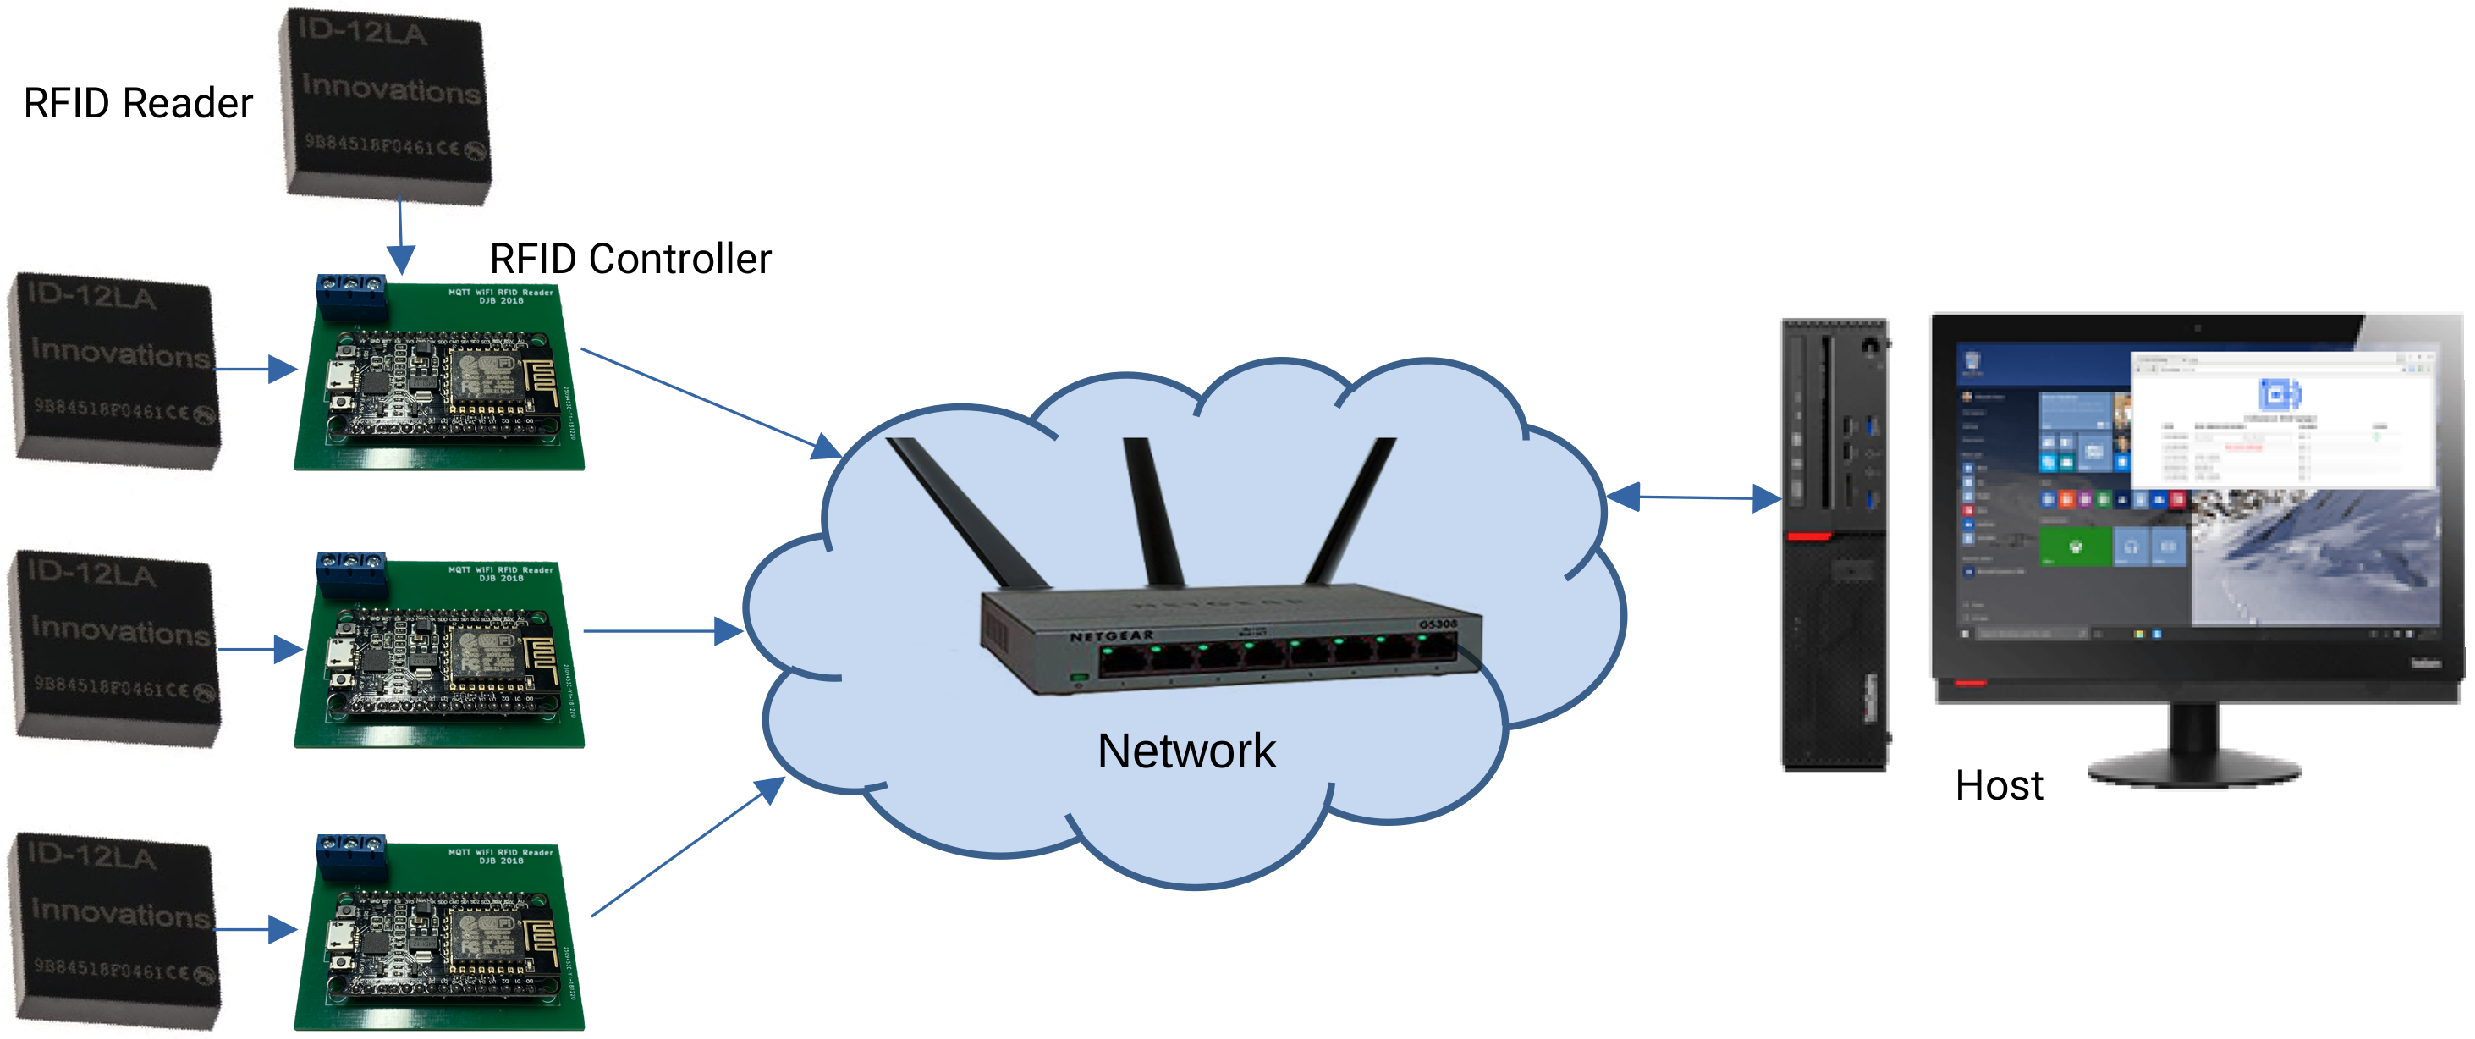
\includegraphics[scale=0.15]{../Images/rsms_system.png}
	\caption{RSMS System Components}
	\label{fig:rsms-system}
\end{figure}

\section{MRLM System Components}

Figure \ref{fig:mrlm-ms-components} depicts the micro-services used to create the \gls{mrlm} subsystem and figure \ref{fig:turnout-system} depicts it's logical architecture.

\begin{figure}[H]
	\centering
		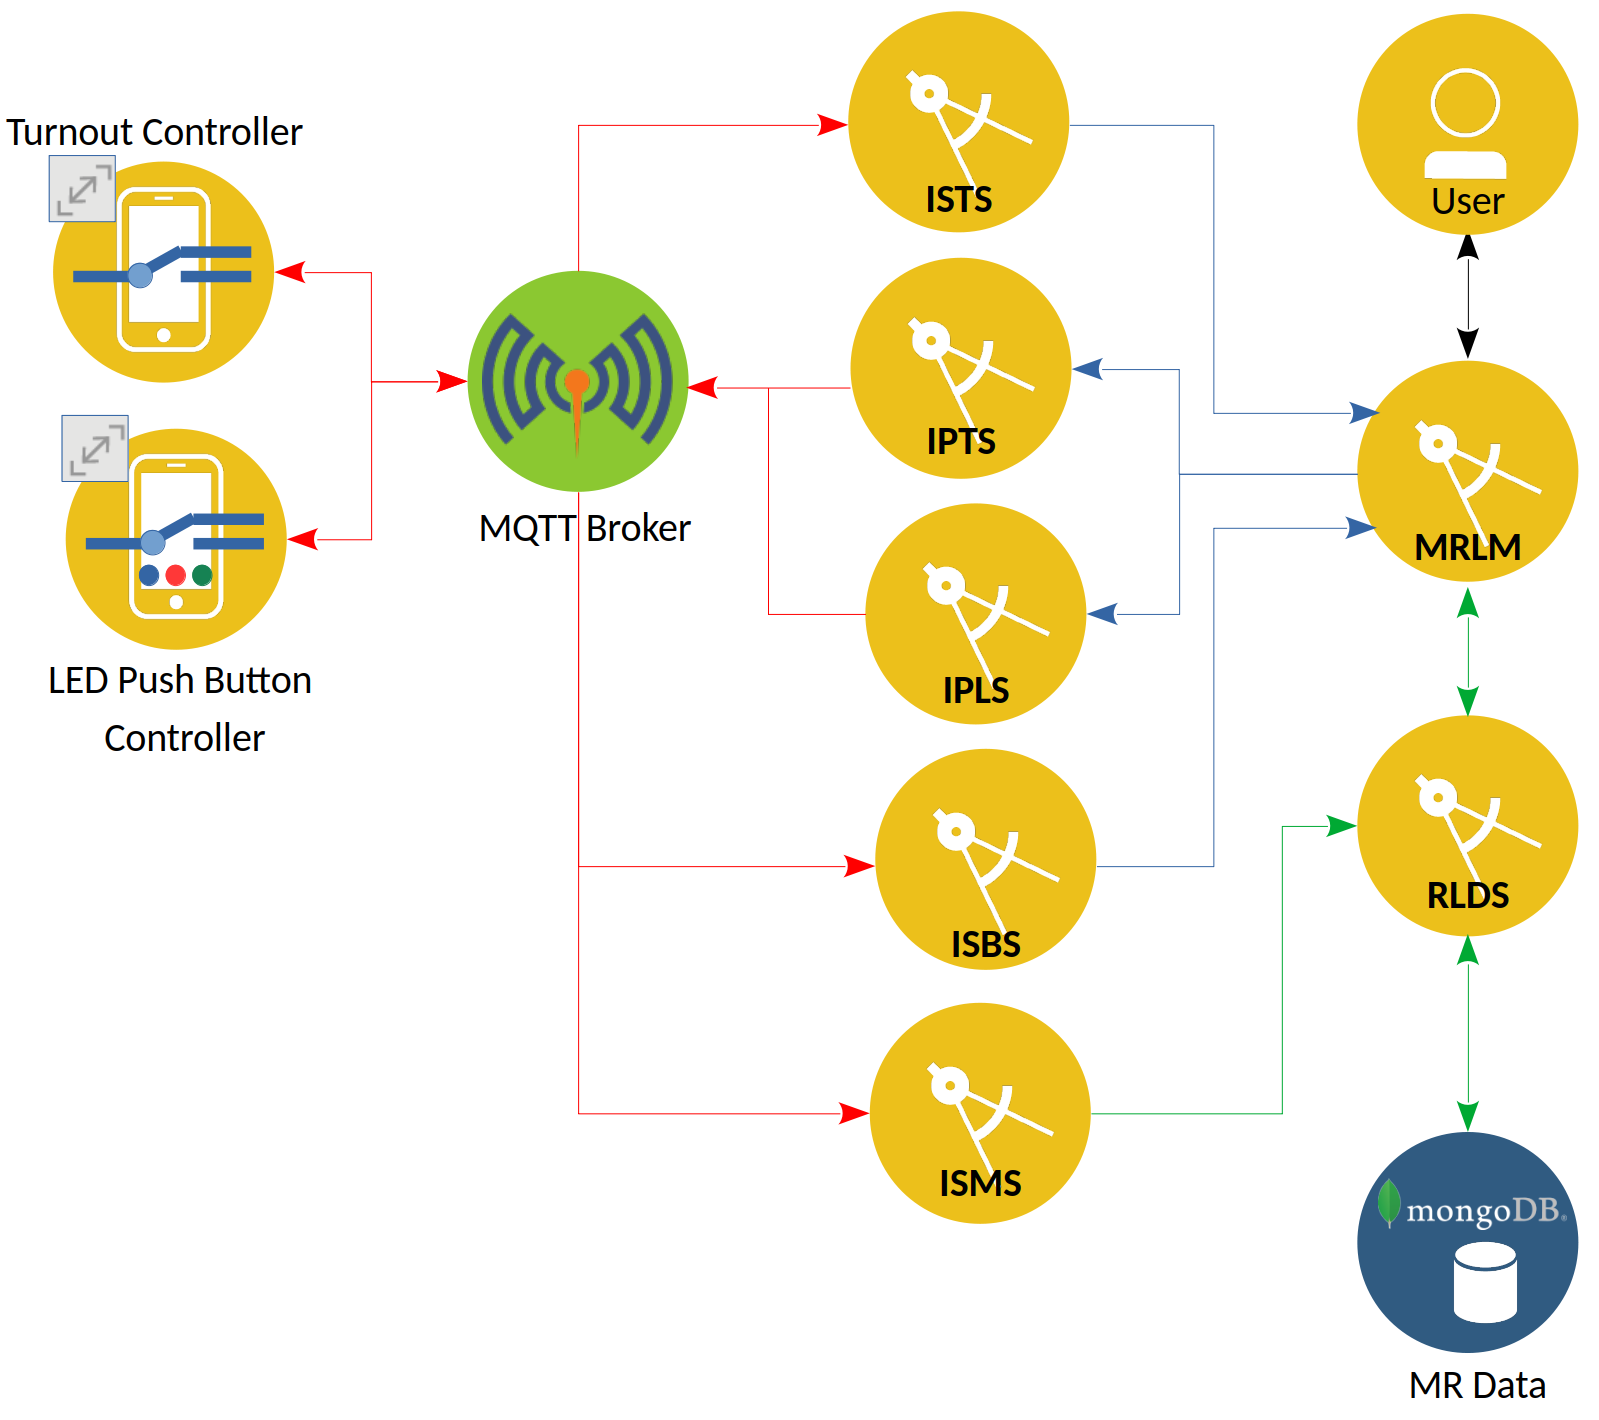
\includegraphics[scale=0.2]{../Images/mrlm_microservices.png}
	\caption{Microservices Components}
	\label{fig:mrlm-ms-components}
\end{figure}


\begin{figure}[H]
	\centering
		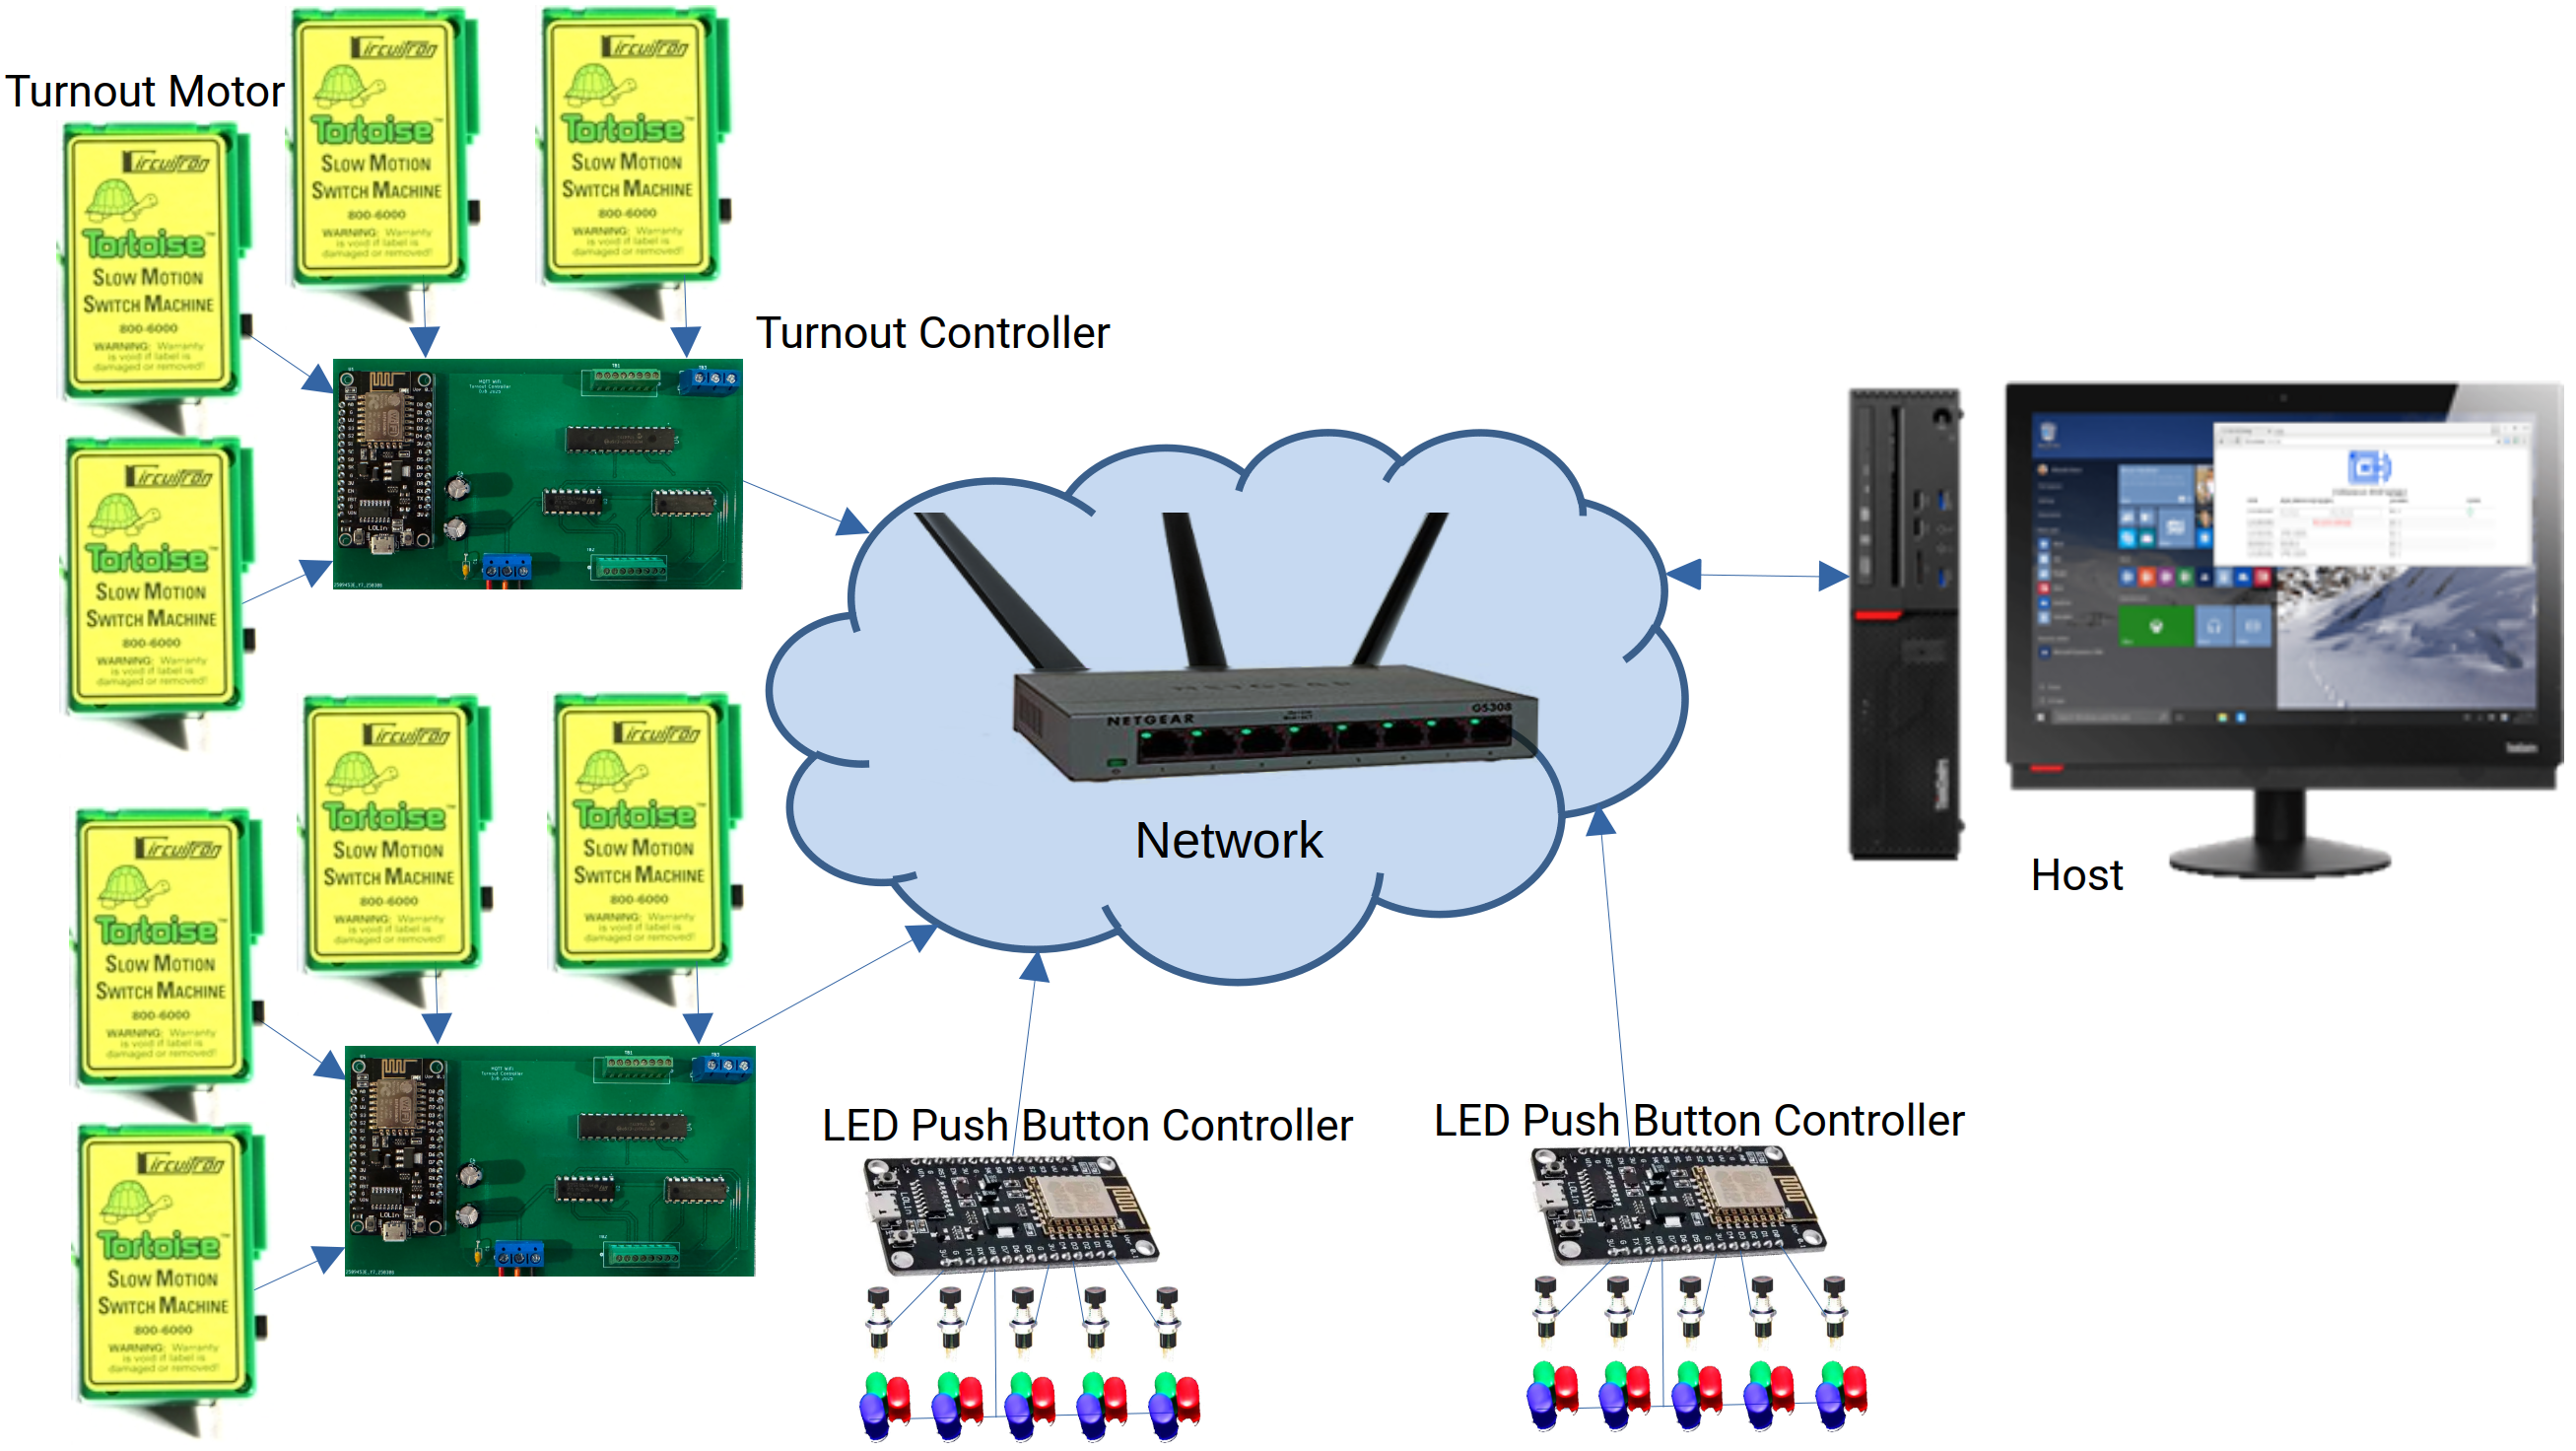
\includegraphics[scale=0.2]{../Images/mrlm_system.png}
	\caption{MRLM System Components}
	\label{fig:turnout-system}
\end{figure}

\chapter{Use Case Survey Model}
A use case survey model is a method of identifying and documenting the specific tasks and activities that a particular group of users (such as modelers or operators) performs with a product or system. The goal of a use case survey is to understand how the users interact with the product or system, and to identify opportunities for improvement or potential areas of confusion or frustration. The survey typically includes a series of questions that ask the users to describe their tasks and activities, as well as any problems or issues they have encountered. The results of the survey are then analyzed to identify patterns and trends, which can be used to inform design and development decisions.\vspace{5mm} \\
Use cases are used in software development to describe how a system or product should behave in response to certain inputs or events. They provide a clear and detailed understanding of the requirements for a system, and serve as a communication tool between developers, stakeholders and users. These are depicted as ellipses in the survey model.\vspace{5mm} \\
Some of the key benefits of using use cases include:
\begin{itemize}
  \item They help to identify the specific functional requirements of a system, which can be used to guide the design and development process.
  \item Use cases provide a clear and detailed description of how a system should behave in response to different inputs, which can be used to test the system and ensure that it meets the requirements.
  \item Use cases can be used to identify and document the different types of users and their specific needs, which can be used to inform user-centered design decisions.
  \item They provide a clear and consistent way to communicate the requirements of a system to different stakeholders, including developers, business analysts, and project managers.
  \item Use cases can be used to identify potential risks and problems early in the development process, which can help to minimize the impact of these issues on the overall project.
\end{itemize}
In use case modeling, an actor is a person or system that interacts with the system being developed. Actors represent the external entities that interact with the system in order to achieve a specific goal or accomplish a specific task.\vspace{5mm} \\
Each actor is typically defined by a set of characteristics, such as their role, responsibilities, and the specific tasks or activities they perform with the system. Actors can be either human users or other systems that interact with the system being developed.\vspace{5mm} \\
In the use case diagram, actors (human) are represented by stick figures and actors (systems) are represented by subsystem packages. Actors are usually connected to the use cases they interact with by an arrow.\vspace{5mm} \\
Use case actors are important because they help to identify the different types of users or systems that interact with the system, which can be used to inform user-centered design decisions. Actors also help to identify the specific requirements of the system, which can be used to guide the development process and ensure that the final product meets the needs of all stakeholders.\vspace{5mm} \\
Figure \ref{fig:use-case} depicts the use case survey model used to design and develop \ac{RAILS}.
In figure \ref{fig:use-case} the line color:
\begin{itemize}
  \item blue indicates the actor use case relationship
  \item orange indicates an inheritance relationship where the open arrow is the inherited.
  \item purple indicates a uses relationship where the open arrow is the used use case.
\end{itemize}
\begin{figure}
	\centering
		\includegraphics[scale=0.55]{use-case.eps}
	\caption{Use Case Survey Model}
	\label{fig:use-case}
\end{figure}
\section{Actors}
\subsection{Human Actors}
\begin{itemize}
  \item Dispatcher is responsible to develop an operating session plan in which rolling stock is assigned to consists and those consists are routed and scheduled.
  \item Model Railroad Manager is responsible to establish and maintain railroad network; rolling stock inventory; defining \ac{DCC} parameters for appropriate rolling stock; industries and their cargo types; schedule rolling stock and railroad network components for maintenance; initial operating states for all turnouts, signals and \ac{DCC} components.
  \item Model Railroad Modeler is responsible to create, modify, and dispose of model railroad assets.
  \item Session Operator is responsible to execute part or all an operating session plan, outside of the rail yard, using the system and the \ac{DCC} Subsystem.
  \item Session Supervisor is responsible to supervise the execution of part or all an operating session plan by the Session Operators and Yard Masters. This person may also function as a Session Operator.
  \item Yard Master is responsible to execute part of an operating session plan, by assembling the consists inside the rail yard, using the system and the \ac{DCC} Subsystem.
\end{itemize}
\subsection{Subsystem Actors}
\begin{itemize}
  \item \ac{DCC} Subsystem is responsible to transmit messages to rolling stock equipped with \ac{DCC} receiver/controller, as commanded by the system and to warn the system of possible malfunctions.
  \item Sensor Subsystem is responsible to detect the presence of rolling stock in a railroad network block/segment and provide notification to the system.
  \item Signal Subsystem is responsible to change the state of specified signals located on the rail network as commanded by the system.
  \item Turnout Subsystem is responsible to indicate the state of turnouts on the rail network; change the state of turnouts as commanded by the system; and indicate operators’ action to change the state of turnouts.
  \item Panel Subsystem is responsible for displaying status information about turnouts and providing operator input to change turnout position.
\end{itemize}
\section{Use Cases}
\begin{itemize}
  \item Configure Industries is responsible to establish and maintain the Industry database, allowing the manager to add, modify or delete industries, simulate production/consumption of goods as cargo, and inform the dispatcher of industry cargo requirements.
  \item Control Model Railroad is responsible to assist the operator in managing the execution of an operating session plan. By:
\begin{itemize}
  \item automatically executing the parts of an operating session plan selected by the operator for regular scheduled trains by commanding the Signal, Turnout and \ac{DCC} subsystems; and
  \item assisting the operator executing parts of an operating session plan by commanding the Signal, Turnout and \ac{DCC} subsystems.
\end{itemize}
  \item Configure Maintenance is responsible to establish and maintain the maintenance database, allowing the manager to schedule rolling stock or railroad network components maintenance, simulate component failures, and warn the dispatcher of needed maintenance
  \item Configure Network is responsible to establish and maintain the railroad network database, allowing the manager to add, modify or delete railroad network components, and to initialize the Signal and Turnout Subsystems automatically at startup and as requested by the manager.
  \item Configure Rolling Stock is responsible to establish and maintain the rolling stock database, allowing the manager to add, modify or delete rolling stock and inform the dispatcher of the rolling stock attributes.
  \item Develop Operating Session Plan is responsible to assist the dispatcher in developing an operating session plan.
  \item Dispatch Trains Automatically is responsible for executing the operating session plan autonomously.
  \item Dispatch Trains Manually is reponsible to assist the operators execute the operating session plan.
  \item Shutdown Model Railroad is responsible to bring the system down gracefully ensuring the state be stored so that when the system Startup occurs the system returns to the state when the system was shutdown.
  \item Startup is responsible to bring the system up in either a distributed environment or standalone mode.
  \item Track Model Railroad Assets is responsible to establish and maintain the model railroad asset database, allowing the modeler to add, or modify assets and manage modeling projects.
\end{itemize}

\chapter{Microservices Design Components}
Figure \ref{fig:microarchitecture} shows the microservices components that make up the design of \gls{rails}.

\begin{figure}[H]
	\centering
		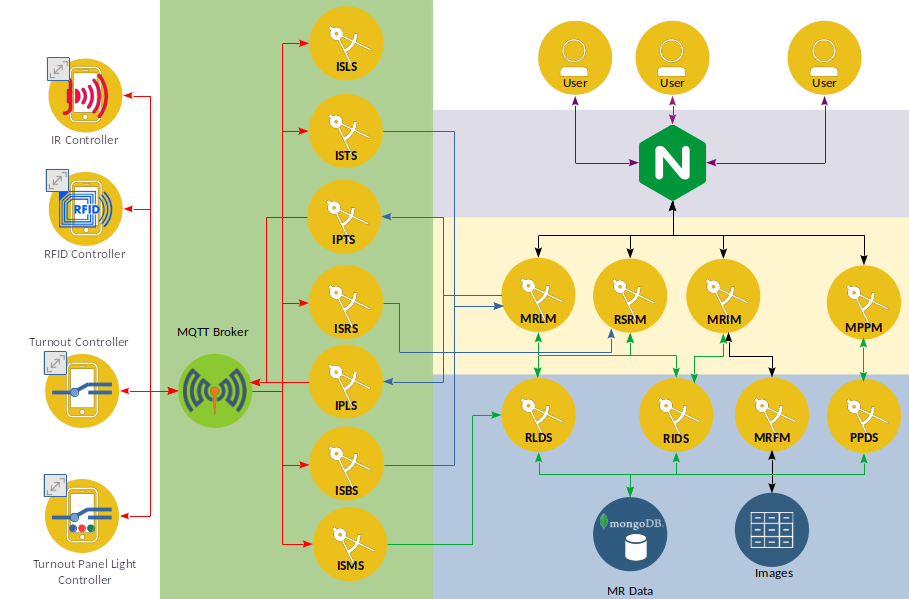
\includegraphics[scale=0.7]{design.png}
	\caption{Microservices Component Architecture}
	\label{fig:microarchitecture}
\end{figure}

The microservices design components are divided into four sets:
\begin{itemize}
  \item \gls{iot} components, which are highlighted with the light green colored background in Figure \ref{fig:microarchitecture}.
  \item \gls{ds} components, which are highlighted with the light blue colored background in Figure \ref{fig:microarchitecture}.
  \item \gls{spa} components, which are highlighted with the buff colored background in Figure \ref{fig:microarchitecture}.
  \item a reverse proxy, which is highlighted with the mauve colored background in Figure \ref{fig:microarchitecture}.
\end{itemize}

\section{\gls{iot} Components}
The components of the \gls{iot} set of design components are subdivided into:
\begin{itemize}
  \item Micro Controllers using the \gls{mqtt} protocol:
\begin{itemize}
  \item \gls{rfid} Controller processes \gls{rfid} tags obtained from a \gls{rfid} reader and then publishes the value
  \item Turnout Controller subscribes to turnout commands then to act on the command to cause the turnout to move. It then publishes the state of the turnout
  \item \gls{ir} Controller (in planning) processes \gls{ir} sensors and publishes their values
\end{itemize}
  \item \gls{mqtt} Broker is the heart of any publish/subscribe protocol, is responsible for receiving messages, posting to designated topics and sending messages to clients subscribing to topics.
  \item The subscribers and publishers bridge the \gls{mqtt} elements with the \gls{gui} applications:
\begin{itemize}
  \item \gls{ipls} publishes turnout panel light commands a Turnout Panel Controller
  \item \gls{ipts} publishes turnout commands to a Turnout Controller
  \item \gls{isbs}  subscribes to push button events and pushes them via a web-socket to the MRLM component
  \item \gls{isls} (in planning) \gls{iot} subscribes to topics that provide location information i.e., \gls{ir} Sensors and \gls{rfid} sensors
  \item \gls{isms} subscribes to micros and adds or updates micros collection in RAILS. It also subscribes to micro heartbeats.
  \item \gls{isrs} subscribes to \gls{rfid} tags and pushes them via a web-socket to the \gls{rsrm} component
  \item \gls{ists} subscribes to turnout switch closures and pushes them via a web-socket to the \gls{mrlm} component
\end{itemize}
\end{itemize}
\section{DS Components}
\gls{ds} consist of all the components that handle and or store the model railroad data:
\begin{itemize}
  \item MR Data – the document repository, MongoDB, to store complete collections of items such as rolling stock, industries (producers and consumers), track elements, turnouts, projects, purchases, etc.
  \item \gls{rids} provides \gls{rest} access to railroad inventory documents
  \item \gls{ppds} provides \gls{rest} access to model railroad projects and purchases documents
  \item \gls{rlds} provides \gls{rest} access to model railroad layout documents
  \item \gls{mrfm} provides the user the ability to upload image files for the use by the \gls{mrim} component
  \item Images is the file store for the images uploaded by \gls{mrfm} component and used by the \gls{mrim} component
\end{itemize}
\section{SPA Components}
\gls{gui} applications that provide user access to RAILS:
\begin{itemize}
  \item \gls{rsrm}, this \gls{spa} allows a user to match a RFID value to a rolling stock road name and number
  \item \gls{mrim}, this \gls{spa} allows a user to create, update and delete model railroad assets, such as rolling stock
  \item \gls{mppm}, this \gls{spa} allows a user to enter information about their projects and purchases
  \item \gls{mrlm}, this \gls{spa} allows a user to enter information about their layout and control elements of it
\end{itemize}
\section{Reverse Proxy}
A server that sits in front of the \gls{spas}, which allows users to access the \gls{spas} from any browser on any \gls{pc} in the network. Using a reverse proxy offers a wide range of practical benefits — from performance and scalability to security and maintainability. However, the principal use of the reverse proxy server in \gls{rails} is to allow multiple browsers on different \gls{pcs} in the same \gls{lan} to view any of the \gls{spas}.


\chapter{IoT Design}

In software architecture, the publish/subscribe pattern is a messaging pattern where senders of messages (publishers), do not program the messages to be sent directly to specific receivers (subscribers), but instead categorize published messages into topics without knowledge of which subscribers, if any, there may be. Subscribers express interest in one or more topics, and only receive messages that are of interest, without knowledge of which publishers, if any, there are. This pattern decouples senders and receivers, allowing for greater scalability and a more dynamic communication environment.\vspace{5mm} \\
Eclipse Mosquitto is an open-source message broker software that implements the \ac{MQTT} protocol, a standard for publish/subscribe messaging for the \ac{IoT}. Mosquitto provides a lightweight way for IoT devices to communicate with each other, allowing them to publish and subscribe to messages on topics. With Mosquitto, devices can publish information, such as sensor readings or status updates, to the message broker and receive updates from other devices. Mosquitto helps to facilitate efficient and effective communication between \ac{IoT} devices in a scalable manner.\vspace{5mm} \\
Table \ref{iot-table} identifies functions excuted by microcontrollers and the \ac{IoT} messaging attributes.\vspace{5mm} \\

\begin{table}[!ht]
    \begin{center}
    \begin{tabular}{|l|l|l|l|}
    \hline
        \textbf{Micro Function} & \textbf{Pub/Sub} & \textbf{Topic} & \textbf{Message} \\ \hline
        RFID Reader & Pub & sensors/rfid & RFID \\ \hline
        Turnout Contacts & Pub & sensors/toc & Turnout\\ \hline
        Turnout Panel Push Button & Pub & sensors/pb & \\ \hline
        Heartbeat & Pub & micros & Micro Info\\ \hline
        Turnout & Sub & acts/to/cntrlr id &  \\ \hline
        Turnout Panel Light & Sub & acts/tpl/cntrlr id &\\ \hline
        Micro Info & Pub & micros & Micro Info\\ \hline
    \end{tabular}
    \caption{\label{iot-table}IoT Micro Function Table}
    \end{center}
\end{table}

Figure \ref{fig:iotdesign} depicts the flow of \ac{MQTT} messages through the \ac{MQTT} broker from and to microservices components.

\begin{figure}[H]
	\centering
		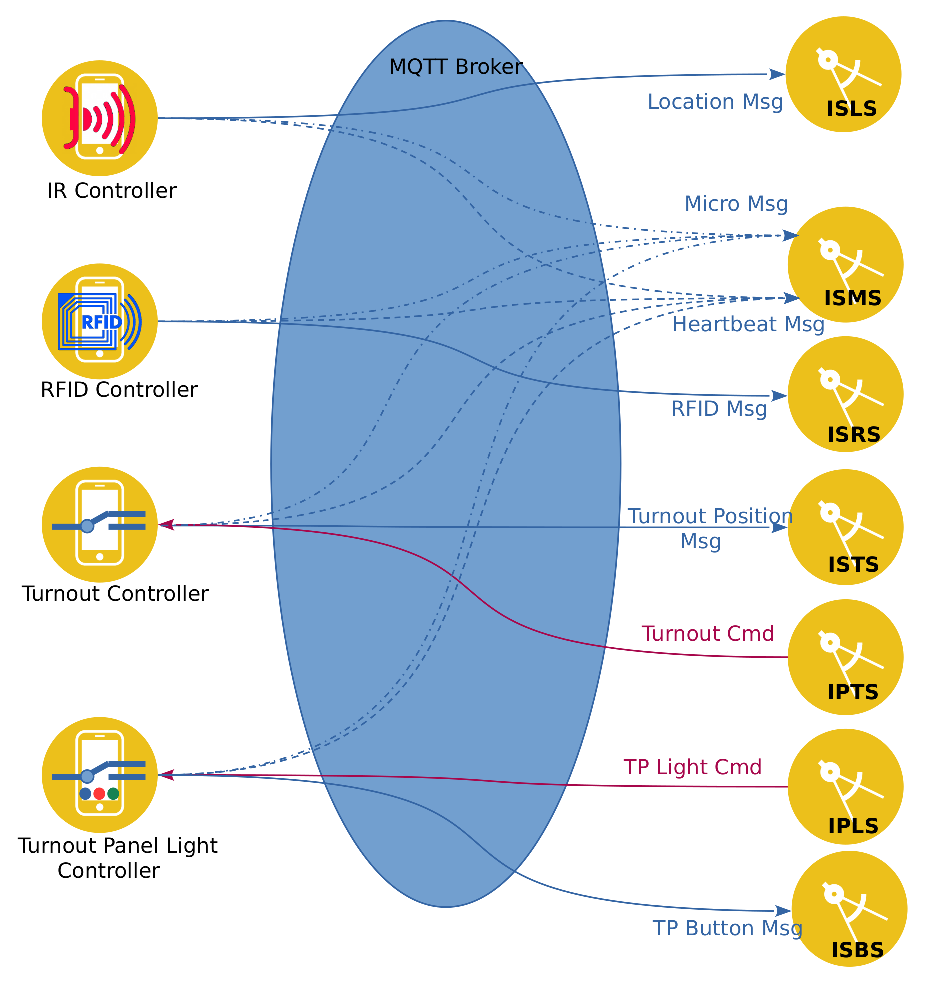
\includegraphics[scale=0.7]{mqtt-v7.eps}
	\caption{IoT Design}
	\label{fig:iotdesign}
\end{figure}

\section{Message Definitions}
\begin{itemize}
\item \ac{RFID} message format: \{“et”:“epoch time",”sensor”:”sensor id“,”rfid”:”rfid tag value“\}
\begin{itemize}
\item example \{"et":"1590463450","sensor":"rfidRdr01","reader":"1","rfid":"1C0044CF23"\}
\end{itemize}
\item\{“et”:”epoch time“,”cntrlr”:”turnout controller id“,”to”:”turnout number“,”state”:”THROWN|CLOSED|ERROR“\}
\item\{“et”:”epoch time“,”cntrlr”:”turnout panel controller id“,”pb”:”push button number“\} 
\item\{“cntrlr”:”turnout controller id“,”to”:”turnout number“,”cmd”:”THROW|CLOSE|STATUS“\}
\item\{“cntrlr”:”turnout panel controller id“,”tpl”:”light number“,”color”:”RED|GREEN|BLUE“,”type”:”BUTTON”\}
\item Micro Info message format: \{“et”:”epoch time“,”sensor”:”sensor id“,"msgType":"initial|heartbeat","ip":"Address of Micro"\}
\begin{itemize}
\item 'heartbeat' example: \{"et":"1590462747","sensor":"rfidRdr01","msgType":"heartbeat"\} 
\item 'initial' example: \{"et":"1590462747","sensor":"rfidRdr01","msgType":"initial","ip":"192.168.0.19"\}
\end{itemize}
\end{itemize}



%%========================================================================
\backmatter

\chapter{Acronyms}
\begin{acronym}
\acro{API}{Application Program Interface}
\acro{CLI}{command-line interface}
\acro{DCC}{Digital Command and Control}
\acro{DS}{Data Services}
\acro{EJB}{Enterprise Java Bean}
\acro{GUI}{Graphic User Interface}
\acro{IDE}{Integrated Development Environment}
\acro{I/O}{input/output}
\acro{IR}{Infrared}
\acro{IoT}{Internet of Things}
\acro{IPLS}{IoT Publisher Turnout Panel Light Services}
\acro{IPTS}{IoT Publisher Turnout Services}
\acro{ISBS}{IoT Subscriber Turnout Panel Button Services}
\acro{ISLS}{IoT Subscriber Location Services}
\acro{ISMS}{IoT Subscriber Micro-controller Services}
\acro{ISRS}{IoT Subscriber RFID Services}
\acro{ISTS}{IoT Subscriber Turnout Services}
\acro{JEE}{Java Enterprise Edition}
\acro{JSF}{JavaServer Faces}
\acro{MQTT}{Message Queuing Telemetry Transport}
\acro{MRFM}{Model Railroad File Manager}
\acro{MRIM}{Model Railroad Inventory Manager}
\acro{MPPM}{Model Projects and Purchase Manager}
\acro{MQTT}{Message Queuing Telemetry Transport}
\acro{MRLM}{Model Railroad Layout Manager}
\acro{QoS}{quality of service}
\acro{SPA}{Single Page Application}
\acro{PPDS}{Plans and Purchases Data Services}
\acro{RAILS}{Railway Administration and Information Logical System}
\acro{RDB}{Relational Database}
\acro{RIDS}{Railroad Inventory Data Services}
\acro{RLDS}{Railroad Layout Data Services}
\acro{RFID}{Radio Frequence Identification}
\acro{RSRM}{Rollingstock RFID Manager}
\acro{SOA}{Services Oriented Architecture}
\acro{UI}{User Interface}
\acro{VCS}{version control system}
\acro{VS Code}{Visual Studio Code}
\end{acronym}


\end{document}
